\subsection{Helices}
\noindent
A helix looks like a spring and appears to look like a circle when viewed from the top looking down.
It has the form $\vec{r}(t) = \langle r\cos{t}, r\sin{t}, ct\rangle$ where $a\in\mathbb{R}$. $a$ defines the ``tightness'' between consecutive windings.

\begin{figure}[H]
	\centering
	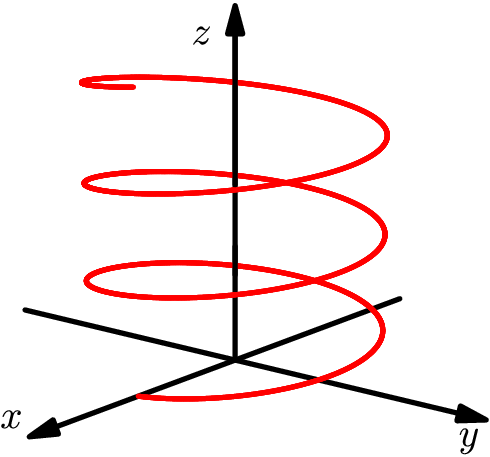
\includegraphics[width=0.5\textwidth]{./Images/vectorValuedFunctions/Helix.png}
	\caption{A helix}
\end{figure}